\documentclass[10pt]{article}
\usepackage{longtable}
\usepackage{float}
\usepackage{wrapfig}
\usepackage{rotating}
\usepackage[normalem]{ulem}
\usepackage{amsmath}
\usepackage{textcomp}
\usepackage{marvosym}
\usepackage{wasysym}
\usepackage{amssymb}
\usepackage{hyperref}
\usepackage{color,soul} % for highlighting
\usepackage{graphicx}
\graphicspath{{/Users/benjaminbass/seacloud/class/earthMaterials/picBank/}}

\usepackage{frame,color}
\usepackage{framed}
\usepackage{minibox}

% \usepackage[T1]{fontenc}
% \usepackage{tilting} %bring title up
% \setlength{\droptitle}{-10cm}

\usepackage[version=3]{mhchem}
% How to Use MChem
% \ce{SO4^2-}
% \ce{^{227}_{90}Th+}
% \ce{A\bond{-}B\bond{=}C\bond{#}D}
% \ce{CO2 + C -> 2CO}
% \ce{SO4^2- + Ba^2+ -> BaSO4 v}


\author{Benjamin Bass}
\date{Date}
\title{\vspace{-2.0cm}Garnet} %bring title up temporary Fix

\begin{document}

\maketitle

% \framebox{Use frameboxes until figure out alignmen}

\begin{center}
  \includegraphics[scale=0.05]{garnet}\footnote{Dodecahedral shape, brown/red color.}
  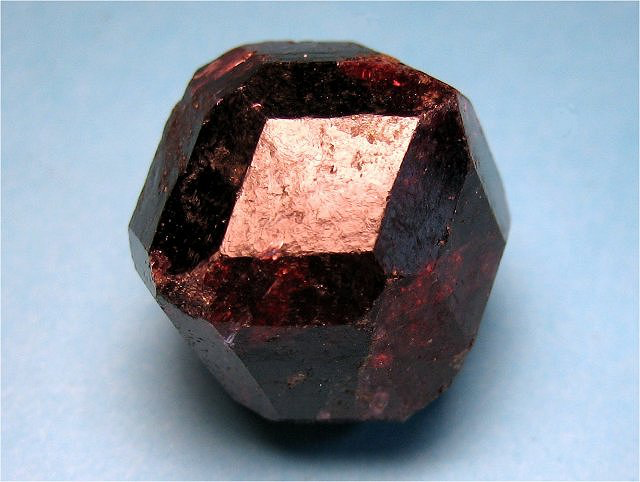
\includegraphics[scale=0.5]{garnet2}\footnote{Up to 8 Hardness. Looks like a prismatic ball.}
\end{center}



\framebox[15cm][l]{\textbf{General Mineral Formula}: $X^{2+}_{3}Y^{3+}_{2}(SiO_{4})_{3}$ }\
\framebox[15cm][l]{\textbf{Mineral Chemical Class}: Nesosilicates}\
\framebox[15cm][l]{\textbf{Specific Gravity}: 3.5-4.3 }\
\framebox[15cm][l]{\textbf{Hardness}: \hl{6.5-8.0} }\
\framebox[15cm][l]{\textbf{Cleavage}: None. May exhibit parting }\
\framebox[15cm][l]{\textbf{Luster}: Vitreous, adamantine, dull }\
\framebox[15cm][l]{\textbf{Streak}: Colorless }\
\framebox[15cm][l]{\textbf{Characteristic Color(s)}: \hl{Red, brown, black, green, yellow, orange, pink, white.} }\
\framebox[15cm][l]{\textbf{Crystal System}: Isometric }\
\framebox[15cm][l]{\textbf{Crystal Class}: 4/m $\overline{3}$ 2/m  }\

\begin{framed}
  \textbf{Crystal Description (common forms, habit, etc.)}: \hl{Well-formed, distinct, dodecahedral and trapexohedral crystals. Also in compact crystal groupings, grainy, massive, and rounded crystals and groups of small crystals.}
\end{framed}

\begin{framed}
  \textbf{Environment (where you find the material}: Metamorphic (Al). Can get garnet when mentmorphize Pelite (sedementary rock) or Mafic rock. If you metamorphie mafic you get (eclogite, blueschist). Mafic like the ocean floor.
Can also get it in sediment. When metamorphic rock weathers.
Can be found in the mantle.
Garnet can be an igneous mineral, but its uncommon.
\end{framed}

\begin{framed}
  \textbf{Common Mineral Associations (in samples, also consult text, notes}: Muscovite, biotite (from pelite). Other individual garnets.
\end{framed}

\begin{framed}
  \textbf{Scientific Usage/Significance}: None
\end{framed}

\begin{framed}
  \textbf{Industrial or Social Use/Significance}: Semiprecious gemstone. Valuable abrasive for sandpaper. Used in filters to help purify water in sanitation plants.
\end{framed}

\begin{framed}
  \textbf{Environmental Significance}: None
\end{framed}

% Possible other Solutions
% \framebox(300,20){\minibox{\textbf{R-Sq}:For example}}

\end{document}
%%% Local Variables:
%%% mode: latex
%%% TeX-master: t
%%% End:
